\documentclass{beamer}
\usepackage[frenchb]{babel}
\usepackage[utf8]{inputenc}
\usepackage[T1]{fontenc}
\usepackage{graphicx}

\usetheme{ENSLyon} 

\title[Adaptation de micro-architectures hétérogènes]{Adaptation de micro-architectures hétérogènes via l'utilisation de gem5 et CERE}
\author[N. Derumigny et P.De Oliveira]{Nicolas Derumigny \and Pablo de Oliveira Castro}
\institute[]{ENS Lyon \hspace*{8em} UVSQ \hspace*{3em}}
\date{5 Septembre 2016}


\usecolortheme{ENSLyon_blue}



\begin{document}



\begin{frame}
	\titlepage
	\begin{center}
	
\includegraphics[height=0.5cm]{logoens.pdf}

	\end{center}
\end{frame}




\section{Introduction}
\begin{frame}
\end{frame}

\section{Outils utilisés}
\subsection{CERE}
\begin{frame}{Codelet Extractor and REplayer : Définitions}
CERE extrait des morceaux de code d'une application, créant ainsi une autre application autonome, reproduisant au plus près possible l'exécution de codelet, autant dans ses instructions que dans son contexte.

\begin{block}{Codelet}
\begin{itemize}
\item Portion d'un application. 
\item \textit{In-vivo} : fonctionnement naturel à l'intérieur de son application.
\item \textit{In-vitro} : fonctionnement de l'application produite par CERE.
\end{itemize}
\end{block}
\end{frame}

\begin{frame}{Fonctionnalités de CERE}
\begin{itemize}
\item Basé sur LLVM.
\item Capture de boucles.
\item Capture de régions OpenMP.
\item Opération au niveau Intermediate Representation (IR).
\item Capture du contexte mémoire précise au pages mémoires près.
\item Deux méthodes de réchauffe du cache : Workload (chargement des données utilisées dans la boucle) et Trace (chargement des derniers accès avant la boucle).
\item Outil de profilage et de mesure du temps du codelet.
\end{itemize}
\end{frame}

\begin{frame}{CERE : Un outil d'isolation de morceaux de code}
\begin{figure}[ht]
\begin{center}
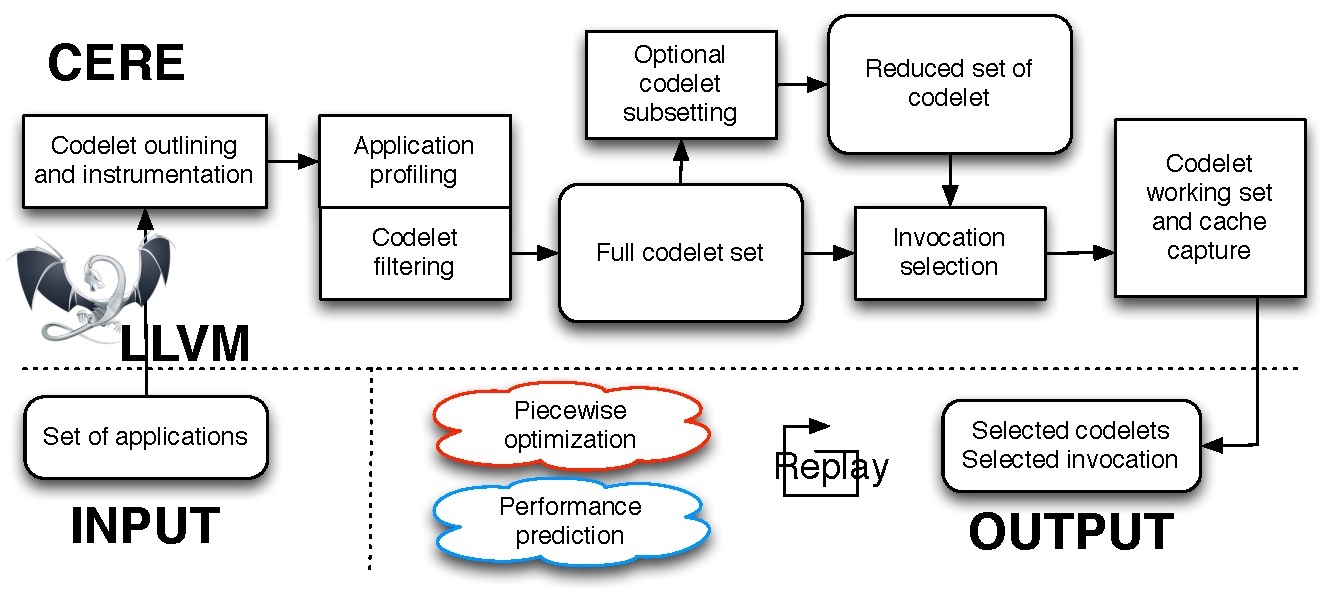
\includegraphics[width=0.85\linewidth]{cere_fonction.pdf}
\caption{\label{CERE_schema}Schéma fonctionnel de CERE.}
\end{center}
\end{figure}
\end{frame}

\subsection{Gem5}
\subsubsection{Généralités}
\begin{frame}{Gem5 : Un simulateur précis au cycle près}
\end{frame}

\subsubsection{Mode d'émulation des appels systèmes}
\begin{frame}{Gem5 : Le mode \textit{syscall emulation}}
\end{frame}


\subsubsection{Mode d'émulation d'un système complet}
\begin{frame}{Gem5 : Le mode \textit{fullsystem}}
\end{frame}


\subsection{McPAT}
\begin{frame}{McPAT : Un simulateur de conception et de consommation de puces}
\begin{figure}[ht]
\begin{center}
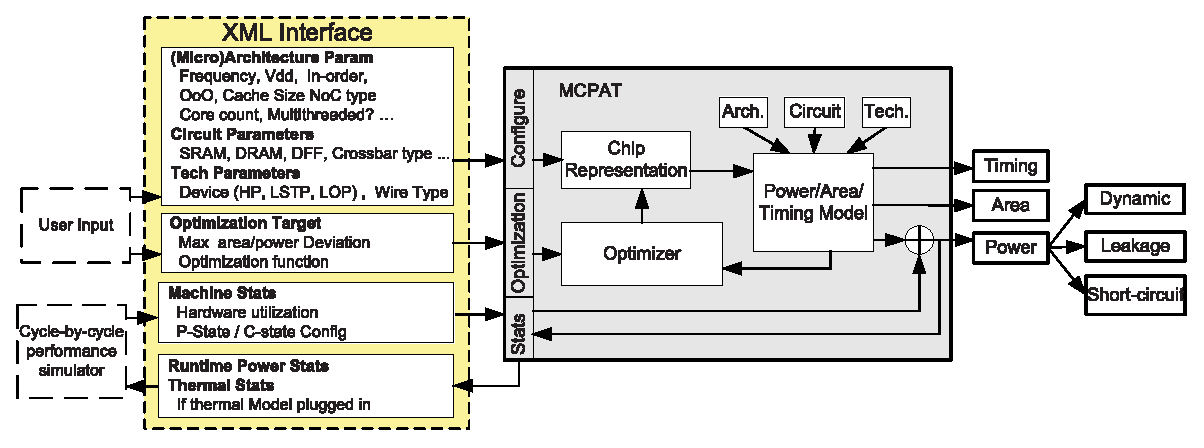
\includegraphics[width=0.84\paperwidth]{McPAT_diag.eps}
\caption{\label{McPAT_schema}Schema fonctionnel de McPAT.}
\end{center}
\end{figure}
\end{frame}


\section{Protocole de simulation}
\subsection{Patch de gem5}
\begin{frame}{Correction de \textit{readFunc()}}

\end{frame}
\begin{frame}{Ajout des appels système \textit{getdents()} et \textit{getdents64()}}
\end{frame}

\begin{frame}{Ajout des appels système \textit{getdents()} et \textit{getdents64()}}
\end{frame}

\subsection{Configuration simulées}
\begin{frame}{Simulation de quatre processeurs aux caractéristiques diverses}
\begin{figure}[ht]
\begin{center}

\begin{tabular}{| l | c | c | c | c | c | c |}
\hline 
& & & \multicolumn{2}{c|}{L2} &\\
Nom & Fréquence & Assoc. & Taille & Assoc. & L3 \\
\hline

A15 & 1 GHz & 2 & 1 Mo & 16 & Non \\

i5-3550 & 3,3-3,7 GHz & 8 & 256 ko & 8 & 8 Mo / 16\\

i5-3337U & 1,8 GHz & 8 & 256 ko & 16 & 4 Mo / 8\\

Q9100 & 2,26 GHz & 8 & 8 Mo & 16 & Non\\
\hline

\end{tabular}
\caption{\label{cpu_setup}Paramètres utilisés pour chaque CPU. Le reste de la configuration est fixe : 8 Go de RAM, processeur x86 générique, et un unique cœur simulé.}
\end{center}
\end{figure}
\end{frame}

\subsection{Codelets choisis}
\begin{frame}{Trois codelets sur le banc d'essai}
\end{frame}

\subsection{Codelets sur Aarch64 ?}
\begin{frame}{Compilation croisée depuis l'architecture x86 vers Aaarch64}
\end{frame}

\section{Résultats}

\subsection{NAS IS}
\begin{frame}{IS : Une première application simple}

\begin{columns}

\begin{column}{0.4\paperwidth}
\begin{figure}
\centering
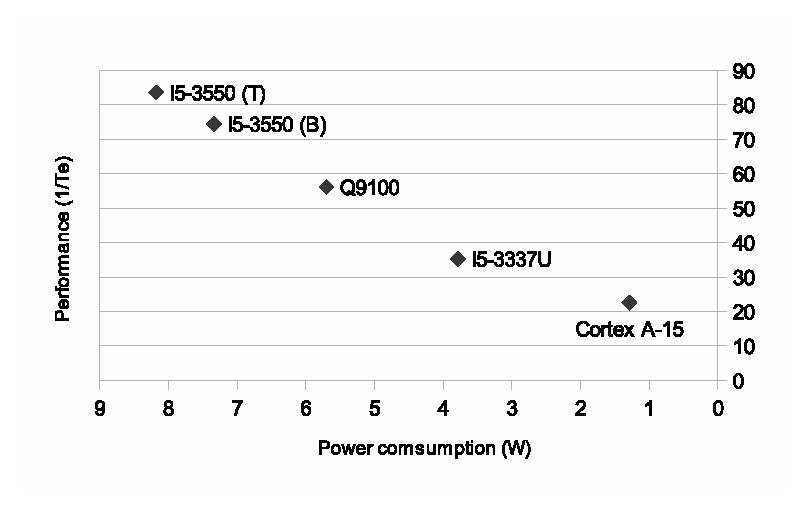
\includegraphics[width=\textwidth]{IS.eps}
\caption{\label{IS}Graphique du ratio performance-consommation énergétique du codelet \textit{IS}.}
\end{figure}
\end{column}

\begin{column}{0.4\paperwidth}
\begin{figure}
\centering
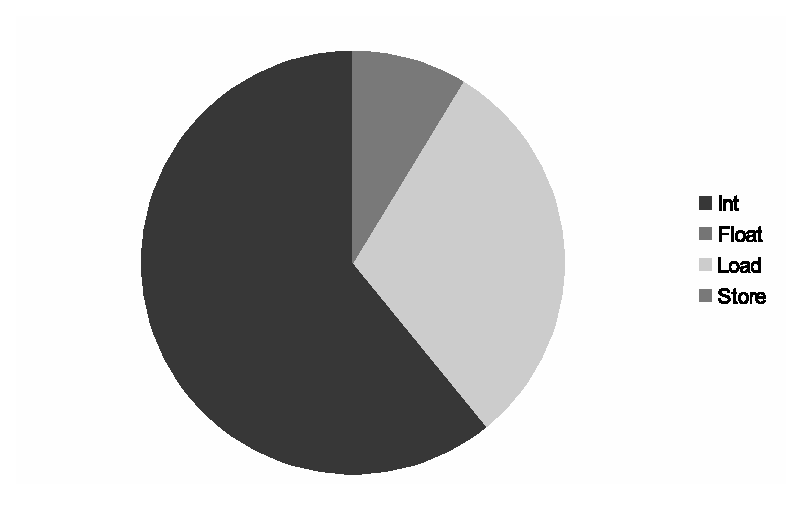
\includegraphics[width=\textwidth]{IS_instr.eps}
\caption{\label{IS_instr}Répartition des instructions au cours de l'exécution du codelet \textit{IS}.}
\end{figure}
\end{column}

\end{columns}

\end{frame}


\subsection{Freqmine}
\begin{frame}{Freqmine : Une application parallèle à peu de données}

\begin{columns}

\begin{column}{0.4\paperwidth}
\begin{figure}
\centering
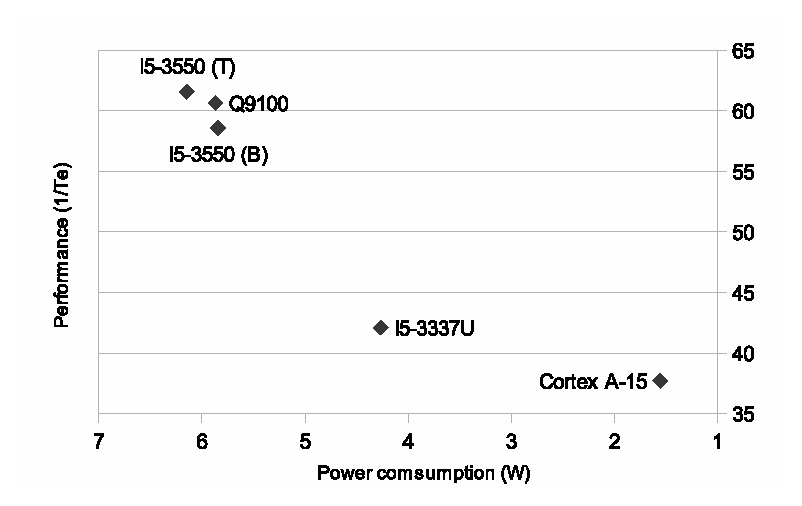
\includegraphics[width=\textwidth]{Freqmine.eps}
\caption{\label{Freq}Graphique du ratio performance-consommation énergétique du codelet \textit{Freqmine}.}
\end{figure}
\end{column}

\begin{column}{0.4\paperwidth}
\begin{figure}
\centering
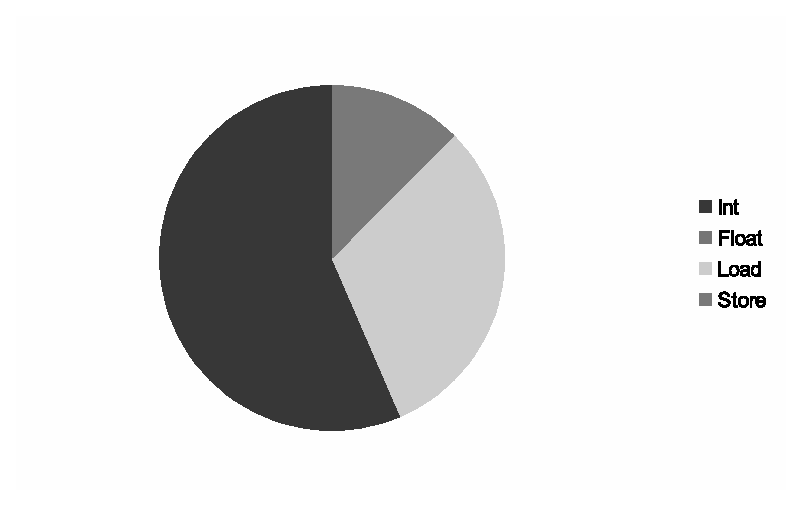
\includegraphics[width=\textwidth]{Freqmine_instr.eps}
\caption{\label{Freq_instr}Répartition des instructions au cours de l'exécution du codelet \textit{Freqmine}.}
\end{figure}
\end{column}

\end{columns}

\end{frame}

\subsection{Blackscholes}
\begin{frame}{Blackscholes : Une application utilisant significativement les flottants}

\begin{columns}

\begin{column}{0.4\paperwidth}
\begin{figure}
\centering
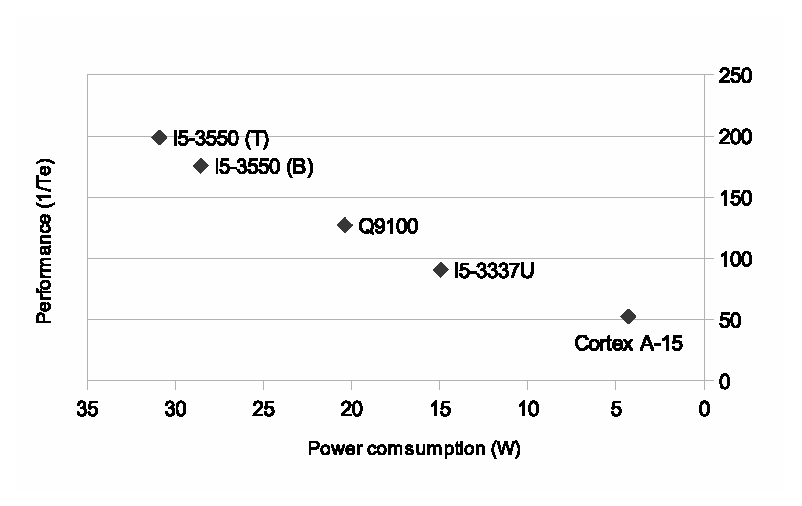
\includegraphics[width=\textwidth]{Blackscholes.eps}
\caption{\label{Blackscholes}Graphique du ratio performance-consommation énergétique du codelet \textit{Blackscholes}.}
\end{figure}
\end{column}

\begin{column}{0.4\paperwidth}
\begin{figure}
\centering
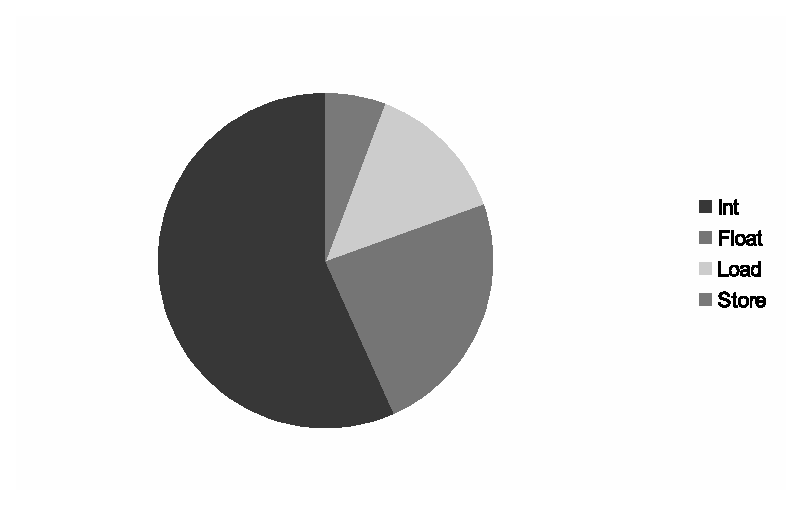
\includegraphics[width=\textwidth]{Blackscholes_instr.eps}
\caption{\label{Blackscholes_instr}Répartition des instructions au cours de l'exécution du codelet \textit{Blackscholes}.}
\end{figure}
\end{column}

\end{columns}

\end{frame}

\begin{frame}{Définition du ratio performance-consommation énergétique}
\begin{block}{Ratio performance-consommation énergétique}
Le ratio performance-consommation énergétique I est défini par :
\begin{equation*}
I=\frac{1}{P.t_e}
\end{equation*}
Avec $P$ la puissance (en W) du processeur simulé et $T_e$ le temps d'exécution du codelet (en s).
\end{block}
\textit{Note :} Cela correspond à l'inverse de la consommation totale du processeur.
\end{frame}

\subsection{Résultats généraux}

\begin{frame}{Graphe récapitulatif}
\begin{figure}
\centering
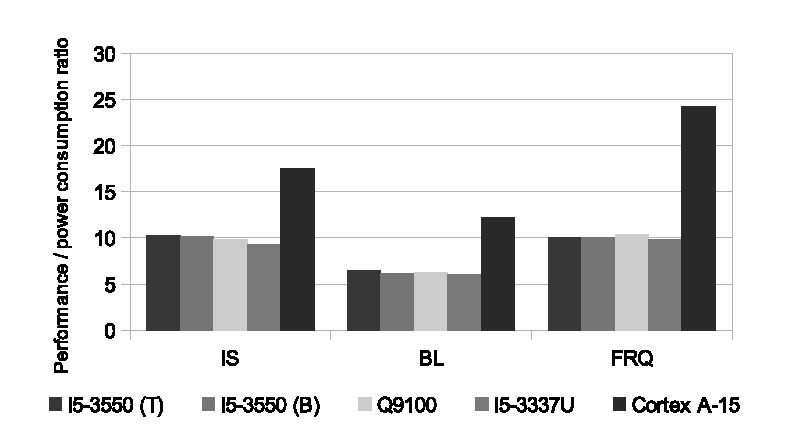
\includegraphics[width=0.65\paperwidth]{Ratio.eps}
\caption{\label{Ratio}Ratio performance-consommation énergétique pour chaque codelet.}
\end{figure}

\end{frame}

\section{Conclusion}
\begin{frame}
\end{frame}

\section{Bibliographie}
\begin{frame}{Bibliographie}
\bibliographystyle{plain}
\bibliography{report}
\end{frame}



\end{document}
